

\section{JMeter}
		I had to choose an application who fitted the needs of our company : 
		a load testing application open source for measuring the performance of its website.

\subsection{Research}
After doing some research, only two applications held my attention : Jmeter and Gatling.


I have chosen Jmeter even though it was difficult to choose. 
Indeeed, I have read both good and bad commentary on the net. 
Jmeter is older than Gatling, hence we can find more tutorial on the  net. 
Moreover, I have read that it is easier to make graphics results on Jmeter, and I was asked to do some graphics analysis.

\begin{figure}[h]
		
\includegraphics[scale=0.5]{Images/JMeter.jpeg} 
		Apache JMeter is a  pure Java application  that can be used as a load testing tool for analyzing
 and measuring the performance of a variety of services. It was originally designed for testing 
 Web Applications but has since expanded to other test functions. 
\end{figure}
	
\subsection{Implementation}
Installing jmetter was not very complex. I just downloaded the release and verified that my 
environment met the requirements (as java 6 or some optional jars (for jdbc, jms..)).
Then it was possible to run the application.\\

I needed to prepare some scenarios. 
Here is an exemple of scenario I registered : 
\begin{enumerate}
	\item click on this link
	\item create a file
	\item and so on.
\end{enumerate}
I wrote a document with some scenario to execute.\\

In order to register scenario, I needed to first configure the browser to use the jmetter
proxy and then I recorded some script tests into jmeter. 
On Jmeter, we need a Test Script Recorder, in order to record every step of our scenario we do on the website.

We also need to add a Thred Group inside the Test Plan, where the scenario will be recorded thanks to the Recording Controller.
And also an HTTP Request Defaults that we configured : set the web server and the port.
Finally, we can start recording.

\subsection{Results}

Once the scenario is recorded, we start to test with the Thread Group.
The following graphism is an example of what we can have after starting the test. 
The scenario consist in creation of files. We can see all the steps in the tree on the left
part. And we can configure some parameters in the right part.\\ 

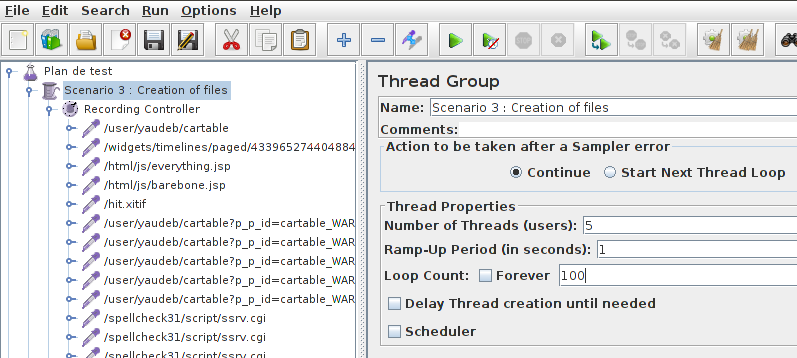
\includegraphics[scale=0.5]{Images/jmetter1.png} 
\\

We set the number of Threads (ex:5) and Loop count (ex:100).
As we can see inside the Recording Controller, a lot of different steps have been recorded. The thred will execute all of them as many times as it is asked to.

We create a summary report to see the results of the execution.

As we can see, it displays every error in each step,  the throughput and so on.

We can also execute some tests with differents users. We write in a file.csv the login and password of some users and add in the application a CSV Data Set Config where we can enter the variables names:LOGIN and MDP (password)  for example.

Then we add the variables inside step of the test. We can see in the tab, near username and password we enter the variables.


It is possible to view some graphics result on Jmeter: \\ 

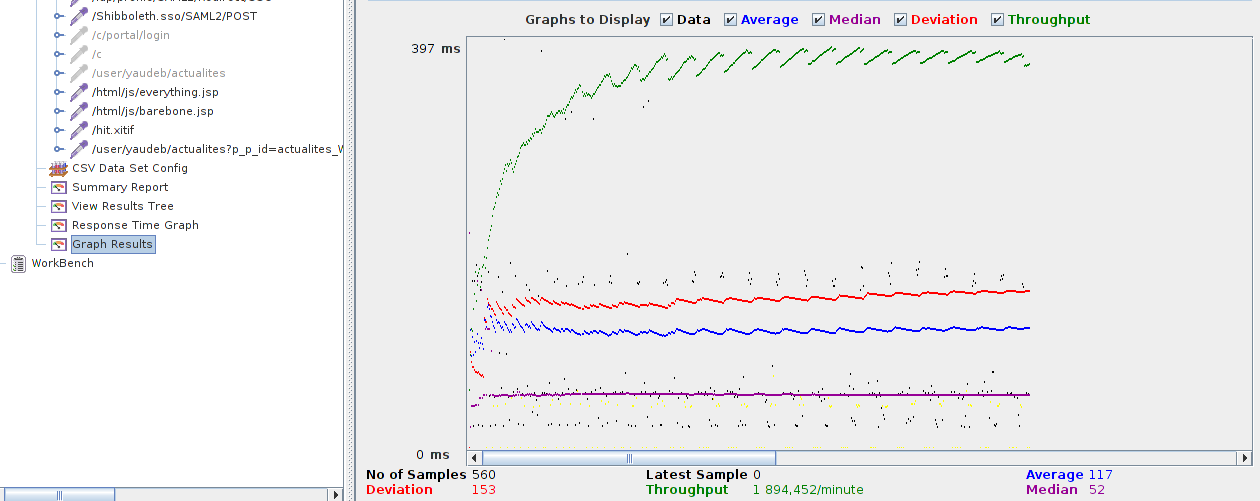
\includegraphics[scale=0.3]{Images/jmetter2.png} 

